\documentclass{beamer}

\usepackage{hyperref}
\usepackage{graphicx}

\setbeamertemplate{caption}{\insertcaption}

\title{Mobile Robot Systems Mini Project 5}
\author{Sam Sully (sjs252), Paul Durbaba (pd452), Luke Dunsmore (ldd25)}
\date{Lent 2020}
	
\begin{document}
		
	\frame{\titlepage}
		
	\begin{frame}
		\frametitle{Project Outline}
		\pause
		\begin{itemize}
			\item<2-> LIDAR based localisation (ex1)
			\item<3-> Improve with range and bearing of other robots (sjs252)
			\item<4-> Centralised approach to world coverage (ldd25)
			\item<5-> Decentralised approach to world coverage (pd452)
		\end{itemize}
	\end{frame}
	\begin{frame}
		\frametitle{Localisation}
		\pause
		\begin{itemize}
			\item<2->Particle filter
			\item<3->LIDAR
			\item<4->Range \& bearing
		\end{itemize}
	\end{frame}
	\begin{frame}
		\frametitle{LIDAR}
		\[
		w_i = \sum_{s_{j} \in \mathrm{Sensors}}\Phi(R(i,j), s_{ij}, \sigma^2)
		\]
		\begin{itemize}
			\item $w_i$ = LIDAR weight of particle $i$
			\item $s_{ij}$ = distance recorded by sensor $j$ on the robot
			\item $\Phi(x,\mu,\sigma)$ = Gaussian PDF with mean $\mu$ and standard deviation $\sigma$ 
			\item $R(i,j)$ = ray traced distance from particle $i$ in the direction of sensor $j$
		\end{itemize}
	\end{frame}
	\begin{frame}
		\frametitle{Range \& Bearing}
		\[
		\bar{w_i} = \sum_{r_j \in N_i}\sum_{p_k \in r_j}\Phi\left(
		\begin{bmatrix}
		D_i(p_k)\\
		\Theta_i(p_k)
		\end{bmatrix},
		\begin{bmatrix}
		d_j\\
		\theta_j
		\end{bmatrix},
		\xi
		\right)
		\]
		\begin{itemize}
			\item $\bar{w_i}$ range \& bearing weight of particle $i$
			\item $N_i$ = robot $i$'s neighbours
			\item $p_k$ ranges over the set of particles from robot $r_j$ \item $d_j$ = received distance between this robot and robot $r_j$
			\item $\theta_j$ = received bearing of this robot from $r_j$
			\item $D_i(p_k)$  = distance between the particle $i$ on this robot and the particle $p_k$ from the other robot
			\item $\Theta_i(p_k)$ = bearing between the particle $i$ and the particle $p_k$ on the other robot
			\item $\xi$ = covariance matrix
		\end{itemize}
		Normalising factors omitted.
	\end{frame}	
	\begin{frame}
		\frametitle{Performance Without Enhancement}
		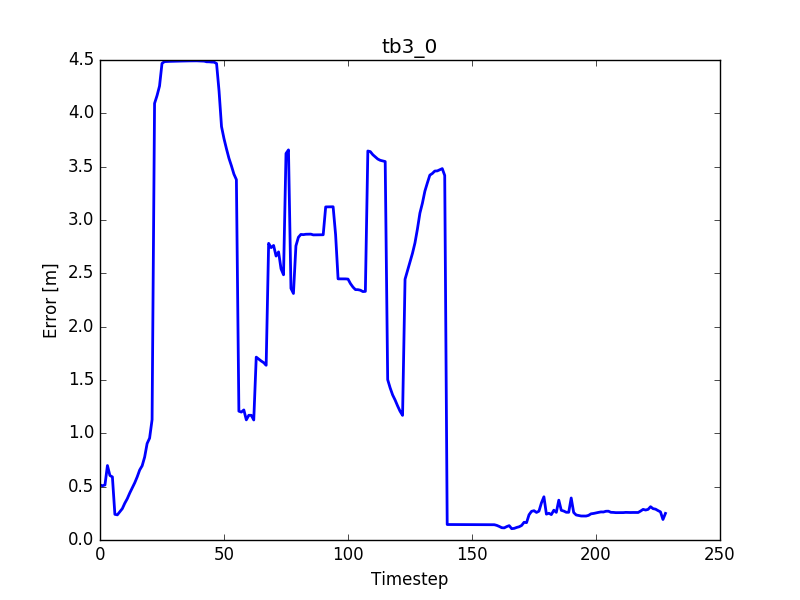
\includegraphics[width=\columnwidth]{figure_l2.png}
	\end{frame}
	\begin{frame}
		\frametitle{Performance With Enhancement}
		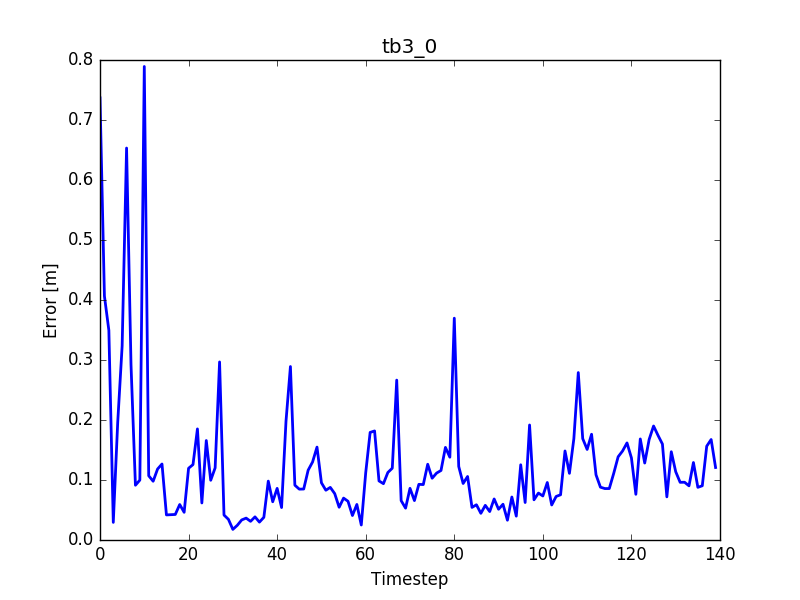
\includegraphics[width=\columnwidth]{figure_l1.png}
	\end{frame}
	\begin{frame}
		\frametitle{Centralised Approach to World Coverage}
		\pause
		\begin {itemize}
			\item<2-> Divide the world into equal regions.
			\item<3-> Plan a path for each robot within its region.
			\item<4-> Follow the paths.	
		\end {itemize}
	\end{frame}
	\begin{frame}
		\frametitle{DARP}
		Divide Areas based on initial Robot Position
		Divide world, $\mathcal{L}$, into regions, $L_i$, such that:
		\begin{itemize}
			\item<2-> $L_i \cap L_j = \phi, \forall i, j  \in 1..n_r, i \neq j$
			\item<3-> $L_1 \cup L_2 \cup \cdots \cup L_{n_r} = \mathcal{L}$
			\item<4-> $|L_1| \approx |L_2| \cdots \approx |L_{n_r}|$
			\item<5-> $L_i$ is connected $\forall i\in 1..n_r$
			\item<6-> $x_i(t_0) \in L_i$ (each robot starts in its own region)
		\end{itemize}
	\end{frame}

	\begin{frame}
		\frametitle{DARP}
		The algorithm:
		\begin{itemize}
			\item<2-> For each robot, weight each cell in the world based on distance to the robot.
			\item<3-> Assign each cell to the robot that gives it the smallest weight.
			\item<4-> Iteratively adjust weights to balance the sizes of the regions and ensure all regions are single connected components.
		\end{itemize}
	
	\end{frame}
	
	\begin{frame}
		\frametitle{DARP}
		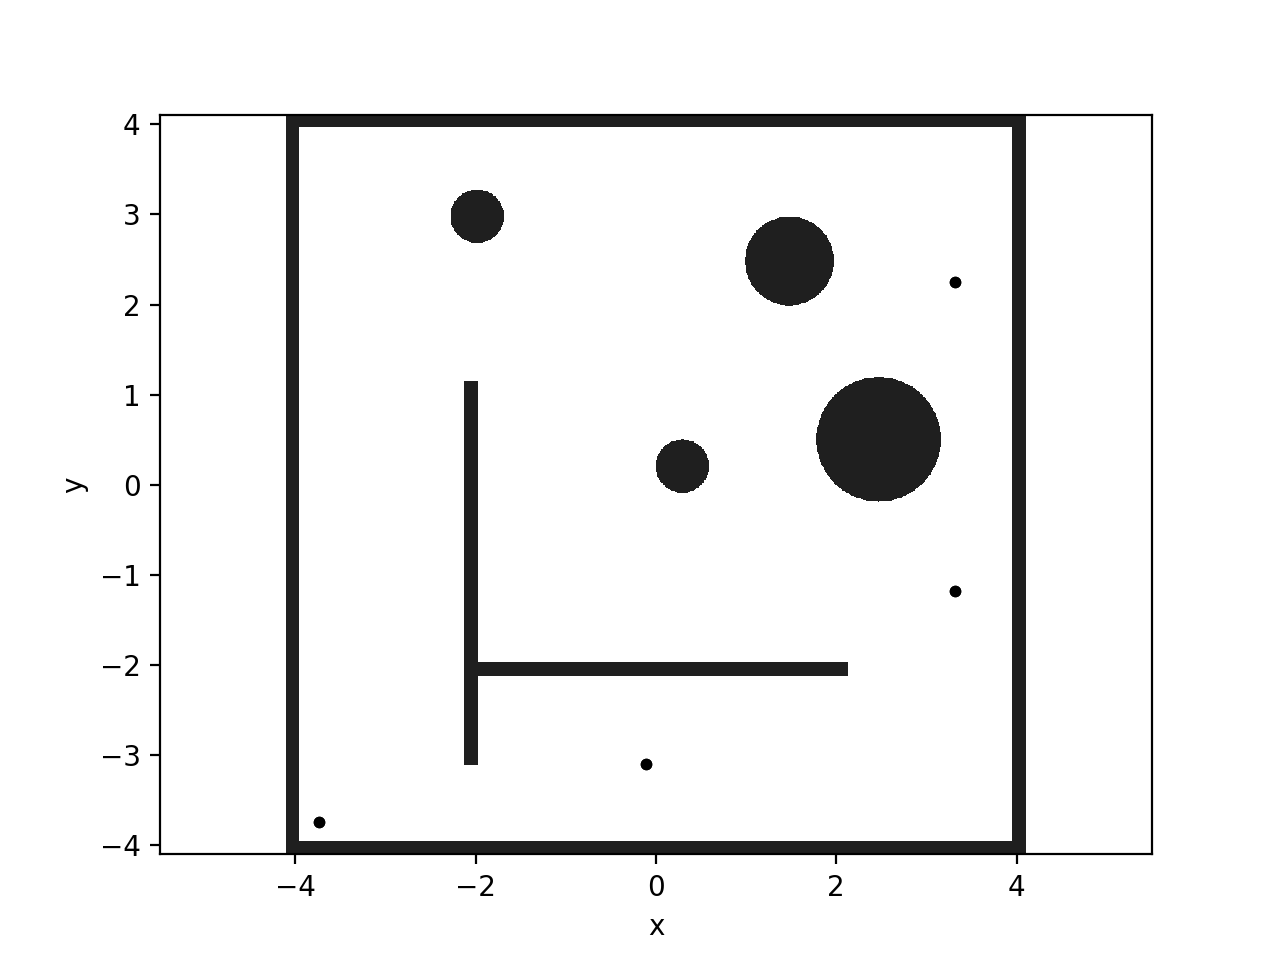
\includegraphics[width=\linewidth]{DARPImages/World_with_robots}

	\end{frame}

	
	\begin{frame}
		\frametitle{DARP}
		\begin{figure}[H]
			\begin{minipage}{0.3\textwidth}
    			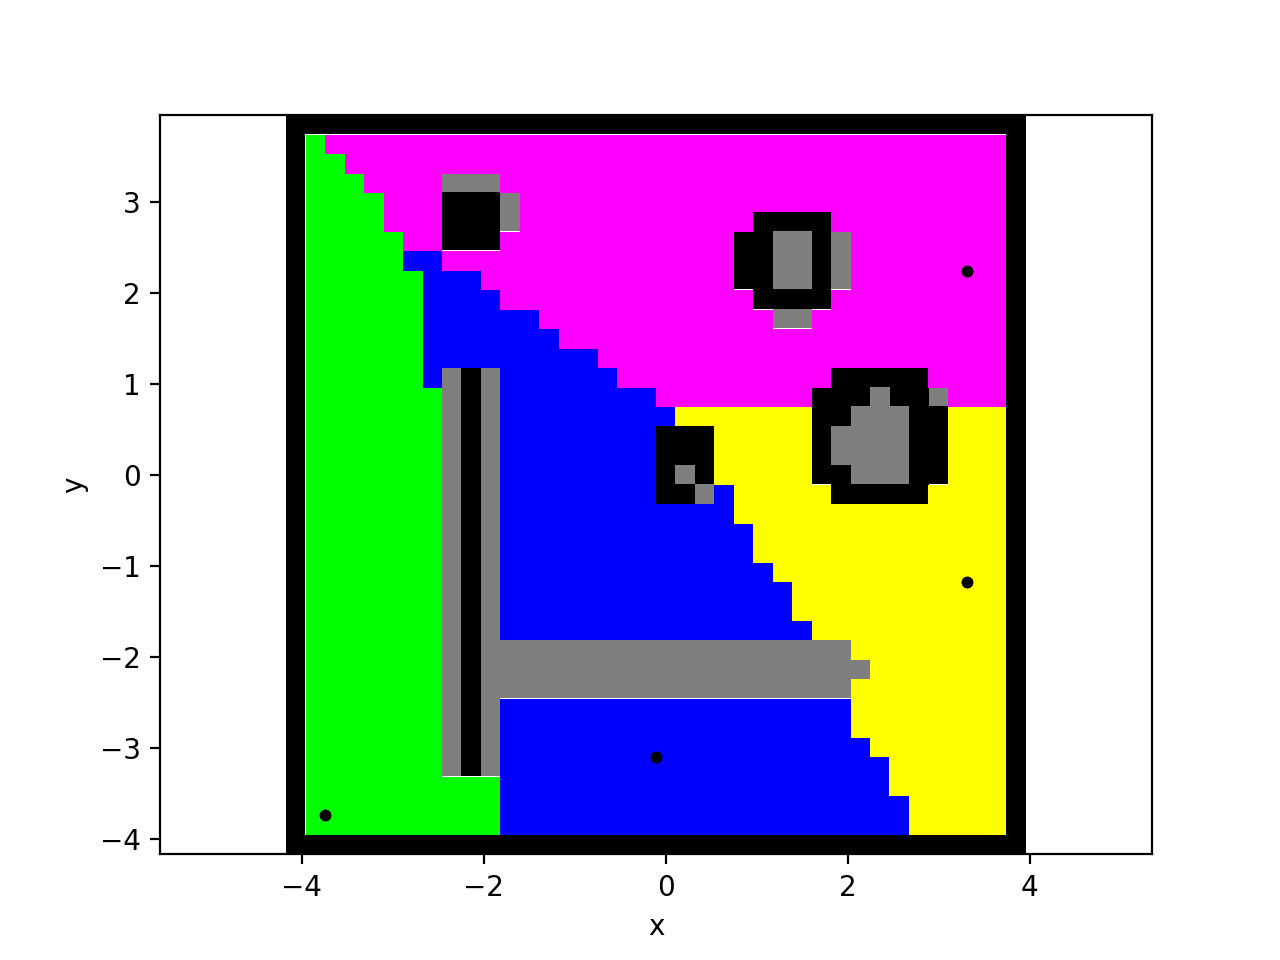
\includegraphics[width=\linewidth]{DARPImages/0}
    			\caption{r=1}
    		\end{minipage}
    		\hspace{\fill} % note: no blank line here
    		\begin{minipage}{0.3\textwidth}
    			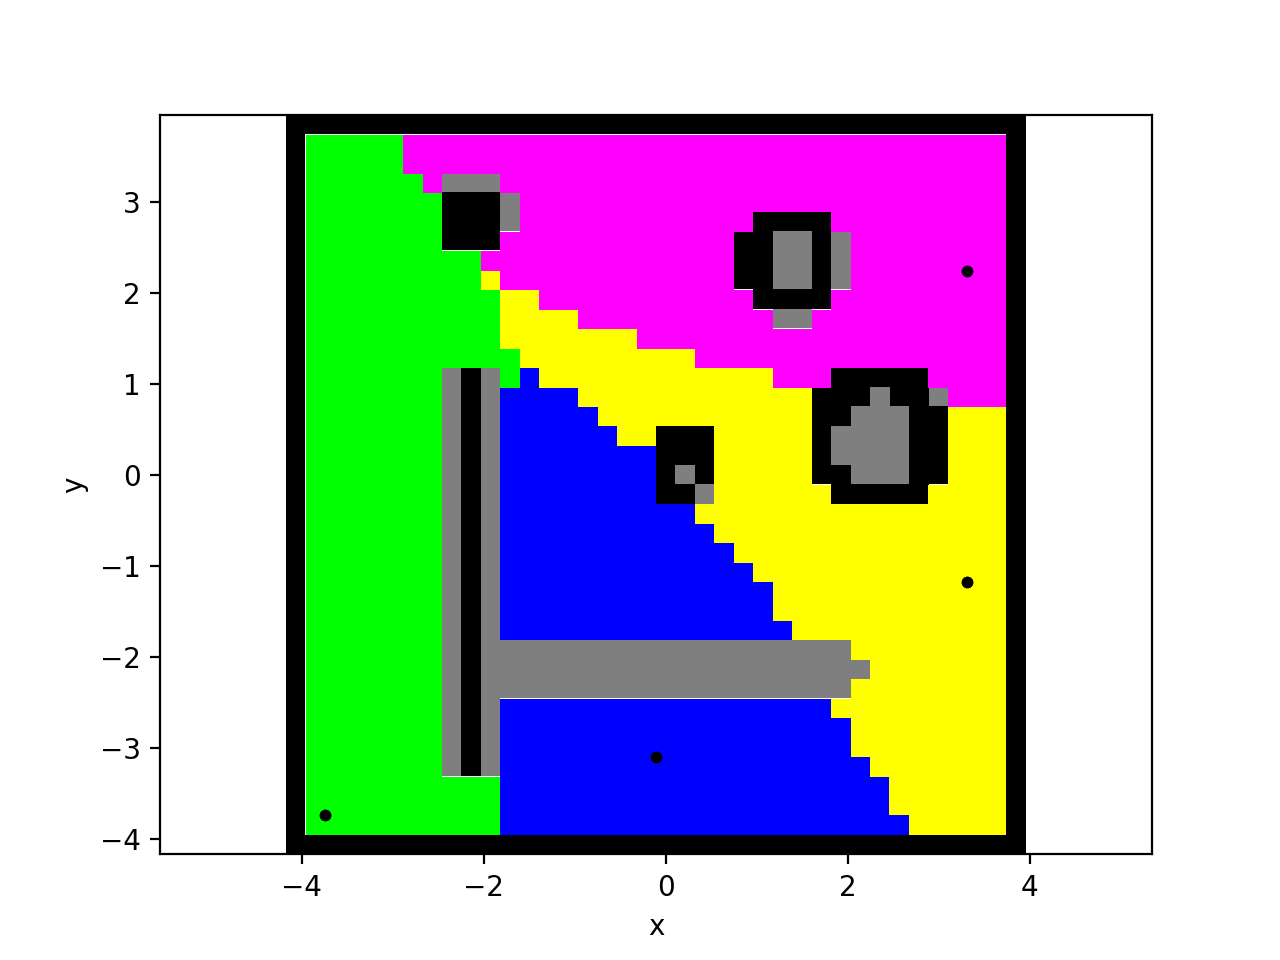
\includegraphics[width=\linewidth]{DARPImages/10}
    			\caption{r=10}
    		\end{minipage}
    		\hspace{\fill} % note: no blank line here
    		\begin{minipage}{0.3\textwidth}
    			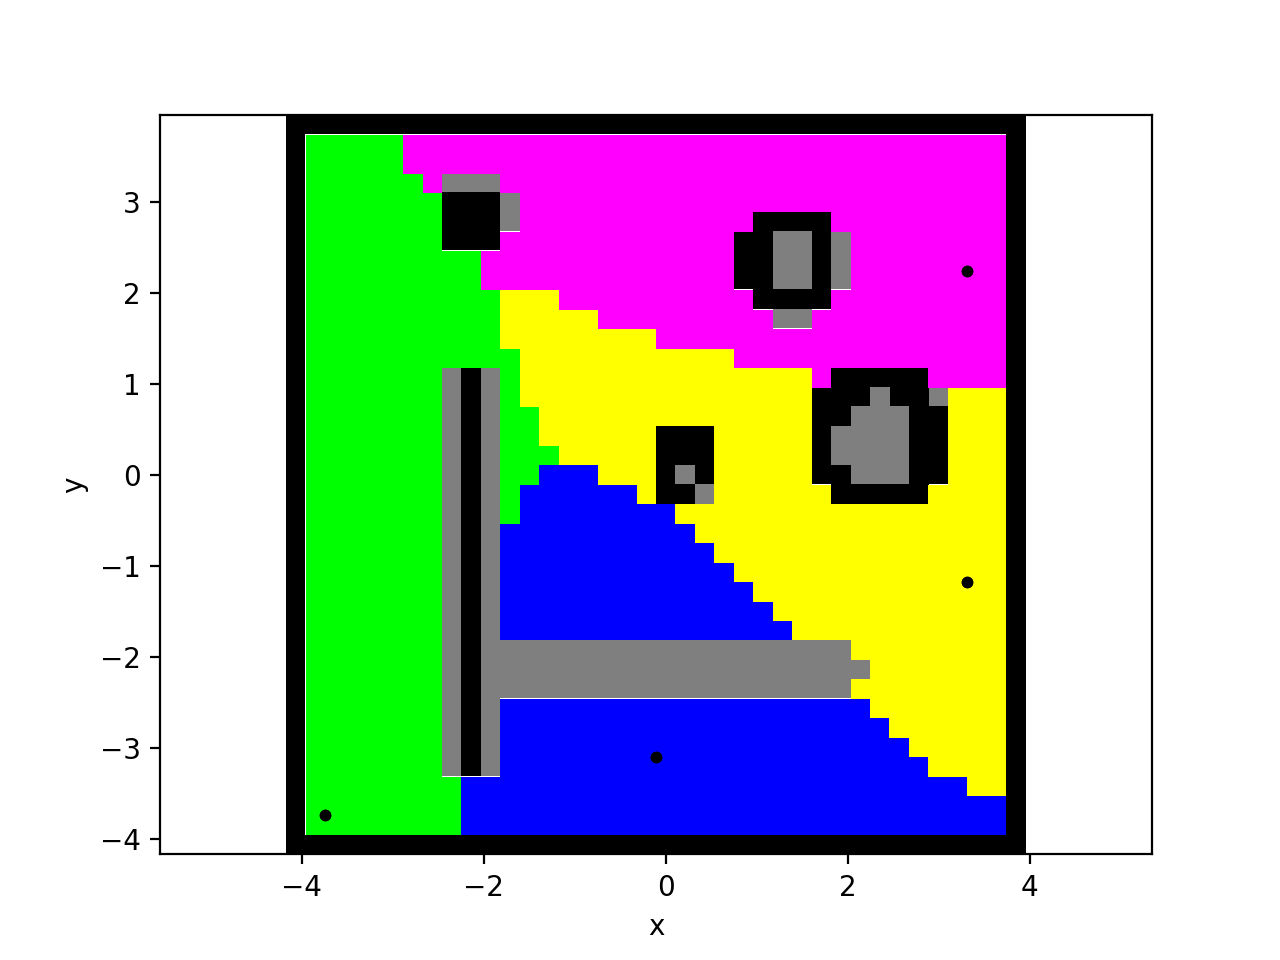
\includegraphics[width=\linewidth]{DARPImages/50}
    			\caption{r=50}
    		\end{minipage}

    		\vspace*{1cm} % vertical separation

    		\begin{minipage}{0.3\textwidth}{}
    			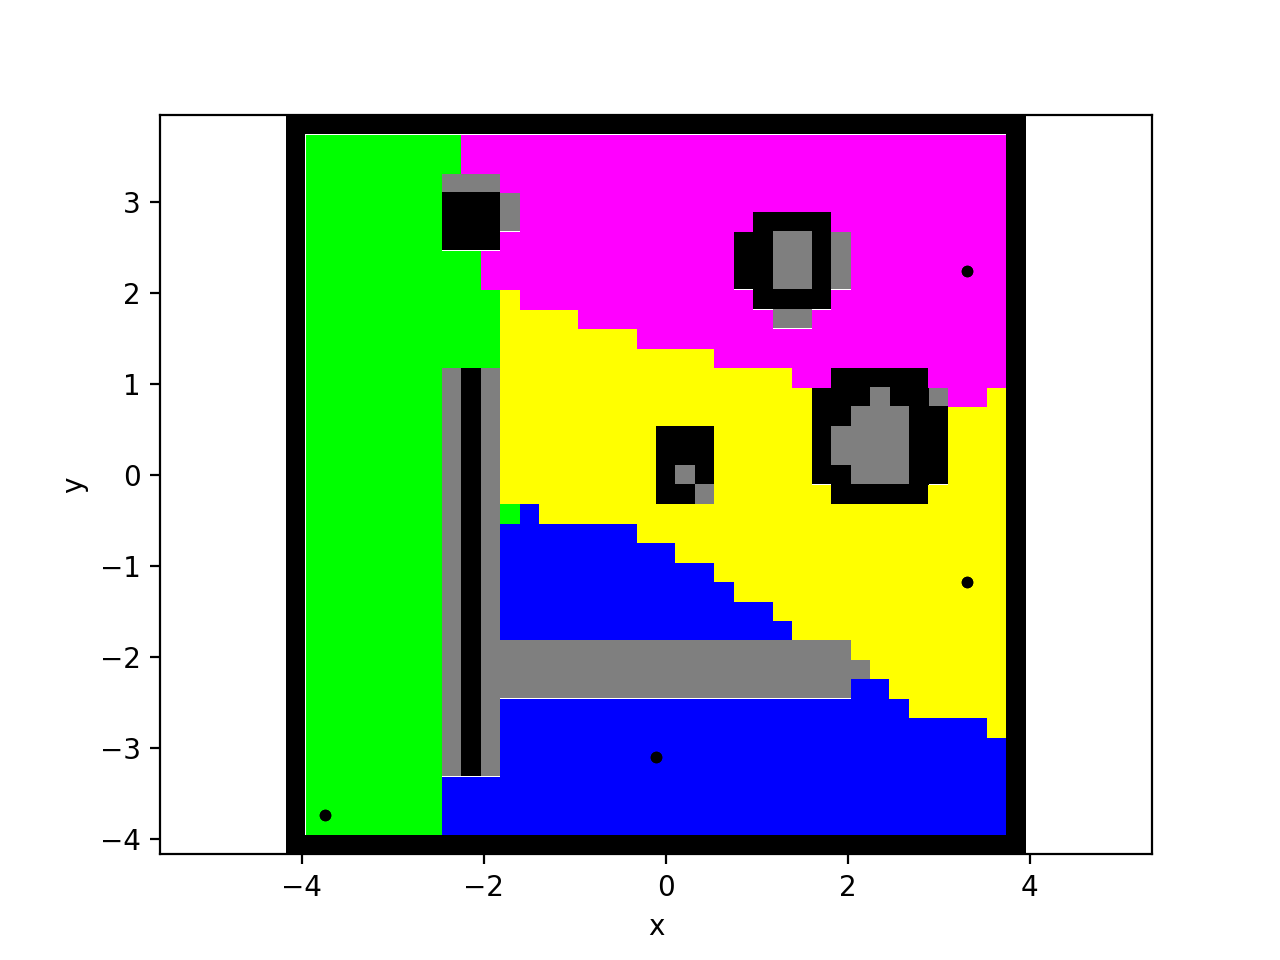
\includegraphics[width=\linewidth]{DARPImages/100}
   				\caption{r=100}
    		\end{minipage}
    		\hspace{\fill} % note: no blank line here
    		\begin{minipage}{0.3\textwidth}
    			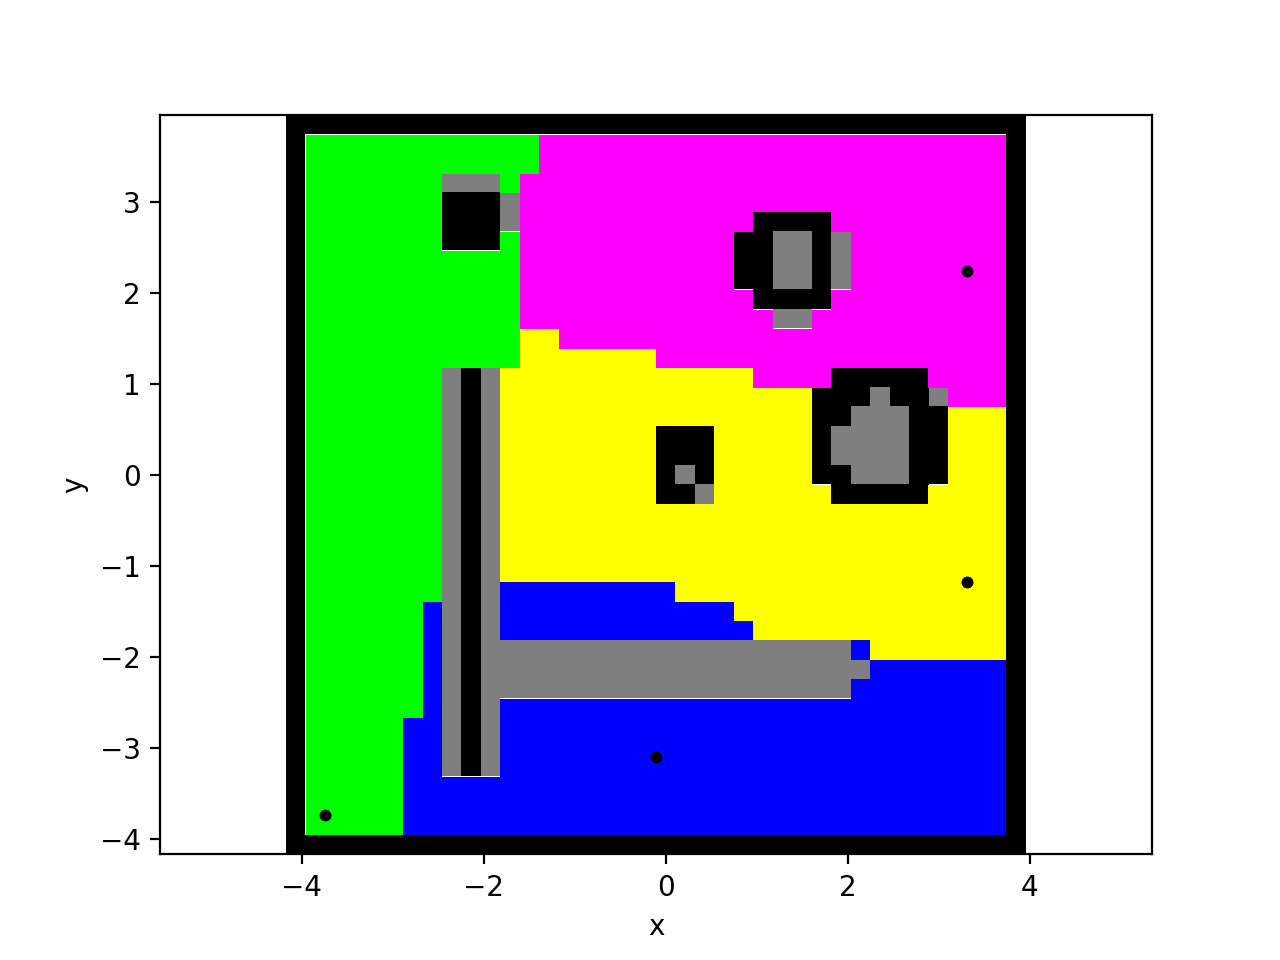
\includegraphics[width=\linewidth]{DARPImages/200}
    			\caption{200}
    		\end{minipage}
    		\hspace{\fill} % note: no blank line here
   			\begin{minipage}{0.3\textwidth}
    			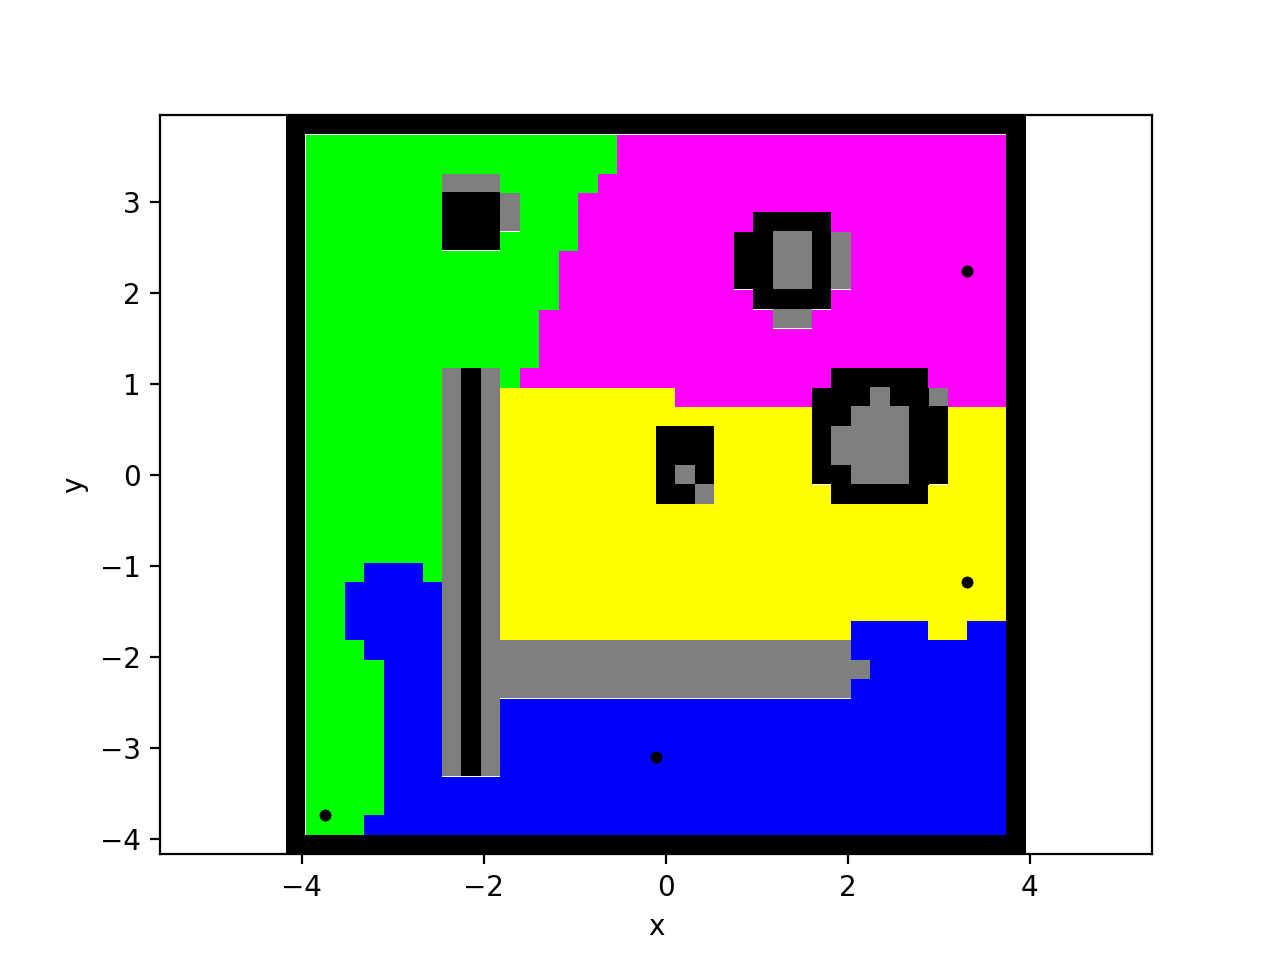
\includegraphics[width=\linewidth]{DARPImages/346}
    			\caption{r=346}
    		\end{minipage}
		
			\caption{Regions after r iterations.} \label{fig:4pics}
		\end{figure}
	\end{frame}
	\begin{frame}
		\frametitle{Path Planning}
		\begin{itemize}
			\item<2-> Each cell is 2x the diameter of the robot.
			\item<3-> For each region, construct a spanning tree between the cells.
			\item<4-> Trace a path around the edges of the spanning tree.
		\end{itemize}
	\end{frame}
	\begin{frame}
		\frametitle{Path Planning}
		\centering
			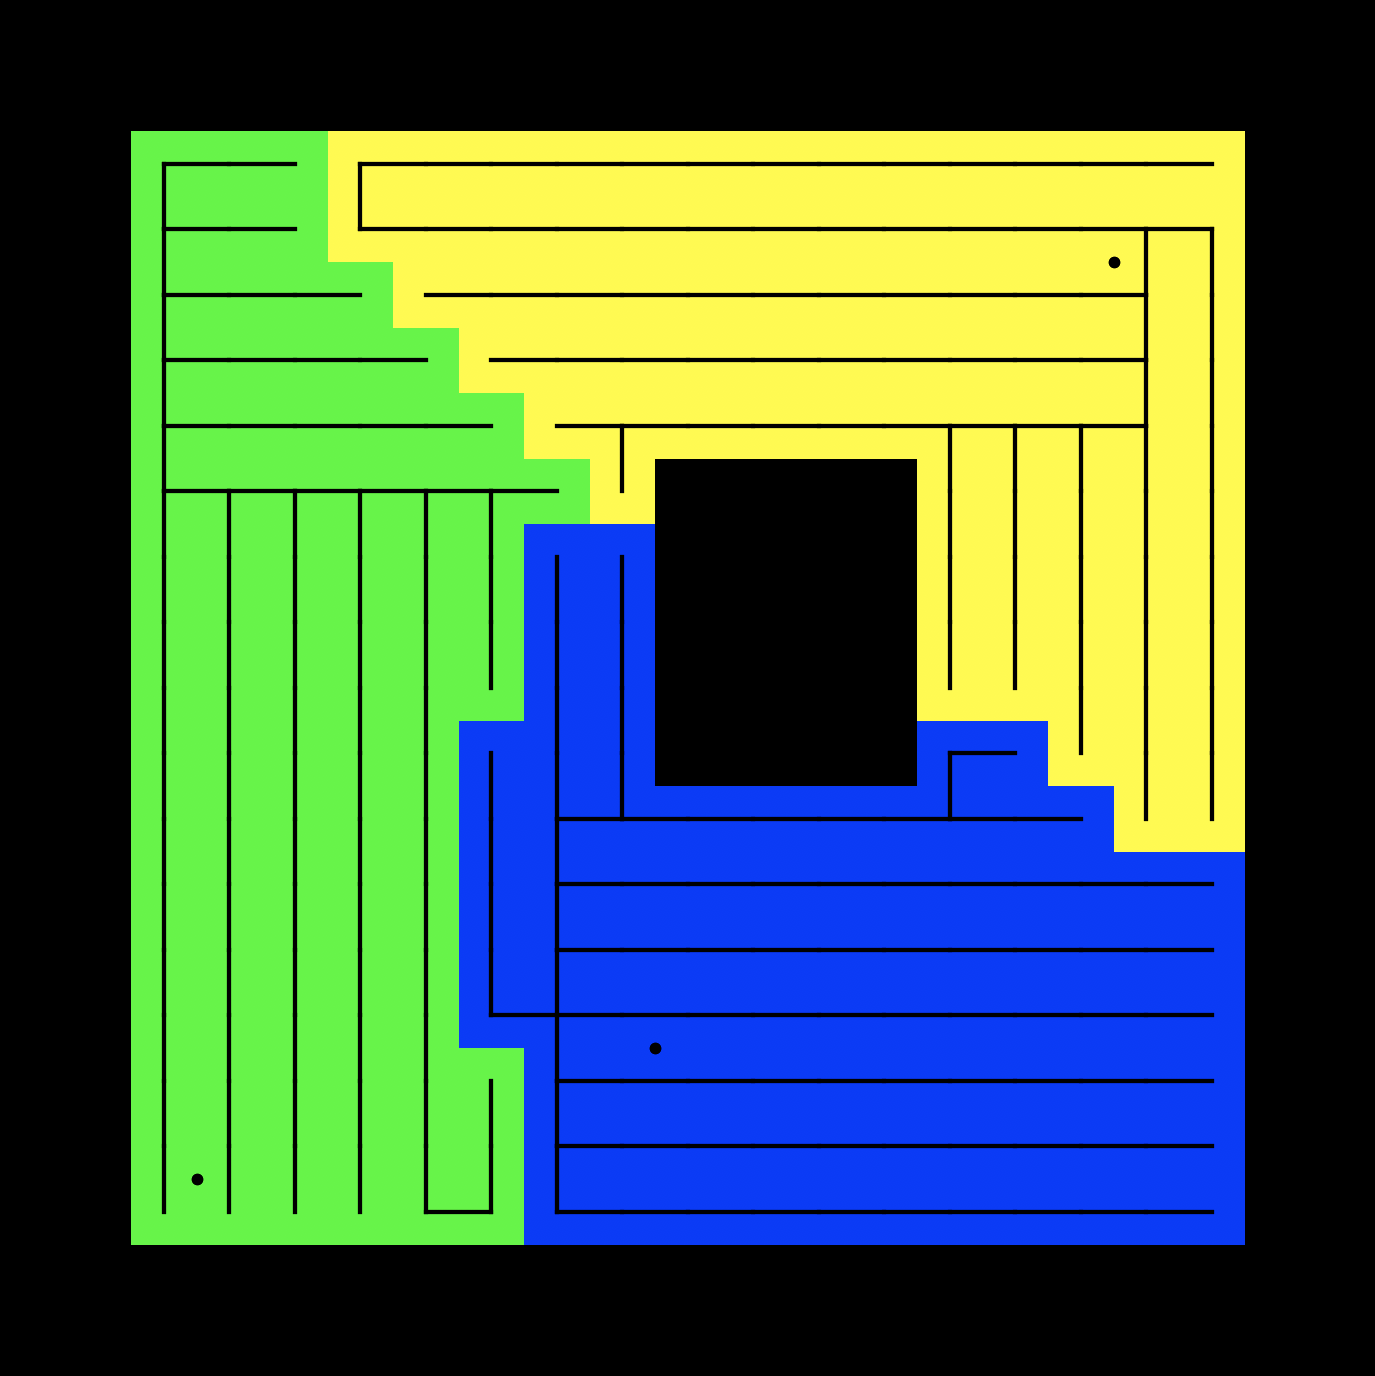
\includegraphics[width=0.7\linewidth]{SpanningTreeExample}
	\end{frame}
	\begin{frame}
		\frametitle{Path Following}
		
	\end{frame}










\end{document}